\documentclass[12pt,letterpaper]{article}
\usepackage{graphicx,textcomp}
\usepackage{natbib}
\usepackage{setspace}
\usepackage{fullpage}
\usepackage{color}
\usepackage[reqno]{amsmath}
\usepackage{amsthm}
\usepackage{fancyvrb}
\usepackage{amssymb,enumerate}
\usepackage[all]{xy}
\usepackage{endnotes}
\usepackage{lscape}
\newtheorem{com}{Comment}
\usepackage{float}
\usepackage{hyperref}
\newtheorem{lem} {Lemma}
\newtheorem{prop}{Proposition}
\newtheorem{thm}{Theorem}
\newtheorem{defn}{Definition}
\newtheorem{cor}{Corollary}
\newtheorem{obs}{Observation}
\usepackage[compact]{titlesec}
\usepackage{dcolumn}
\usepackage{tikz}
\usetikzlibrary{arrows}
\usepackage{multirow}
\usepackage{xcolor}
\newcolumntype{.}{D{.}{.}{-1}}
\newcolumntype{d}[1]{D{.}{.}{#1}}
\definecolor{light-gray}{gray}{0.65}
\usepackage{url}
\usepackage{listings}
\usepackage{color}

\definecolor{codegreen}{rgb}{0,0.6,0}
\definecolor{codegray}{rgb}{0.5,0.5,0.5}
\definecolor{codepurple}{rgb}{0.58,0,0.82}
\definecolor{backcolour}{rgb}{0.95,0.95,0.92}

\lstdefinestyle{mystyle}{
	backgroundcolor=\color{backcolour},   
	commentstyle=\color{codegreen},
	keywordstyle=\color{magenta},
	numberstyle=\tiny\color{codegray},
	stringstyle=\color{codepurple},
	basicstyle=\footnotesize,
	breakatwhitespace=false,         
	breaklines=true,                 
	captionpos=b,                    
	keepspaces=true,                 
	numbers=left,                    
	numbersep=5pt,                  
	showspaces=false,                
	showstringspaces=false,
	showtabs=false,                  
	tabsize=2
}
\lstset{style=mystyle}
\newcommand{\Sref}[1]{Section~\ref{#1}}
\newtheorem{hyp}{Hypothesis}

\title{Problem Set 1}
\date{Due: October 1, 2023}
\author{Liu Yuanyuan}

\begin{document}
	\maketitle
	
	\vspace{1cm}
	\section*{Question 1: Education}

A school counselor was curious about the average of IQ of the students in her school and took a random sample of 25 students' IQ scores. The following is the data set:\\
\vspace{.5cm}


\begin{enumerate}
	\item Find a 90\% confidence interval for the average student IQ in the school.\\
	  \lstinputlisting[language=R,firstline=3,lastline=9]{PS01_Yuanyuan_Liu.R}
	  \begin{itemize}
		\item \textbf{Result}:\\
		 90\% Confidence Interval for School Students' Average IQ:\\
		   93.95993  102.9201  \\
		
       \end{itemize}
	\item Next, the school counselor was curious  whether  the average student IQ in her school is higher than the average IQ score (100) among all the schools in the country.\\ 
	\noindent Using the same sample, conduct the appropriate hypothesis test with$\alpha=0.05$.
		\lstinputlisting[language=R, firstline=12, lastline=23]{PS01_Yuanyuan_Liu.R} 
		\begin{itemize}
	      \item \textbf{Result:}\\
		  Hypothesis Test Results:\\
		  Test Statistic (t): -0.5957439\\ 
		  p-value: 0.7215383 \\
		  we fail to reject the null hypothesis. School students' average IQ is equal to the national average.
	\end{itemize}
\end{enumerate}

\newpage

	\section*{Question 2 (40 points): Political Economy}

\noindent Researchers are curious about what affects the amount of money communities spend on addressing homelessness. The following variables constitute our data set about social welfare expenditures in the USA. \\
\vspace{.5cm}


\begin{tabular}{r|l}
	\texttt{State} &\emph{50 states in US} \\
	\texttt{Y} & \emph{per capita expenditure on shelters/housing assistance in state}\\
	\texttt{X1} &\emph{per capita personal income in state} \\
	\texttt{X2} &  \emph{Number of residents per 100,000 that are "financially insecure" in state}\\
	\texttt{X3} &  \emph{Number of people per thousand residing in urban areas in state} \\
	\texttt{Region} &  \emph{1=Northeast, 2= North Central, 3= South, 4=West} \\
\end{tabular}

\vspace{.5cm}
\noindent Explore the \texttt{expenditure} data set and import data into \texttt{R}.
\vspace{.5cm}
\lstinputlisting[language=R, firstline=30, lastline=31]{PS01_Yuanyuan_Liu.R}  
\vspace{.5cm}
\begin{itemize}

\item
Please plot the relationships among \emph{Y}, \emph{X1}, \emph{X2}, and \emph{X3}? What are the correlations among them (you just need to describe the graph and the relationships among them)?
\vspace{.5cm}
\lstinputlisting[language=R, firstline=32, lastline=35]{PS01_Yuanyuan_Liu.R} 
\begin{figure}[H]
	\centering
	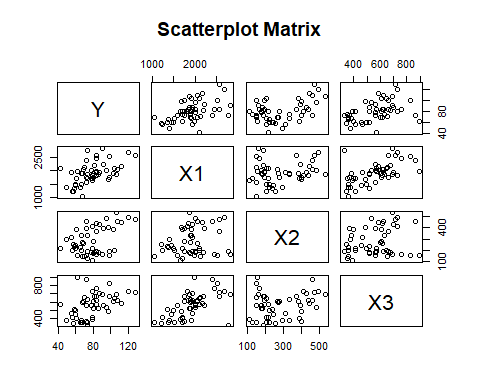
\includegraphics[width=0.8\textwidth]{1}
\end{figure}

		\begin{itemize}
	\item \textbf{Result:}
	\item   relationship between Y and X1 :
	Most of the data points are located near a trend line in the scatterplot matrix, indicating that the correlation between Y and X1 may be strong.
	In the scatterplot matrix, there appears to be some kind of positive linear relationship between Y and X1, with the data points showing a roughly positive correlation trend.
	
	\item  Relationship between Y and X2 :
	Most of the data points also lie near a trend line in the scatterplot matrix, suggesting that the correlation between Y and X2 may be strong.
	There appears to be some sort of negative linear relationship between Y and X2 in the scatterplot matrix, with the data points showing a roughly negative correlation trend.
	
	\item  Relationship between Y and X3 :
	The data points are widely distributed in the graph with no apparent linear relationship, possibly indicating a weak correlation between Y and X3.
	The relationship between Y and X3 in the scatterplot matrix looks much more scattered, with no clear linear trend.
	
	\begin{figure}[H]
		\centering
		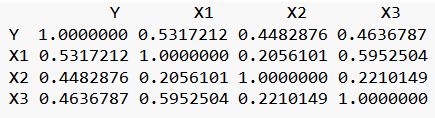
\includegraphics[width=0.8\textwidth]{2}
	\end{figure}
\end{itemize}
\item
Please plot the relationship between \emph{Y} and \emph{Region}? On average, which region has the highest per capita expenditure on housing assistance?
\vspace{.5cm}
\lstinputlisting[language=R, firstline=38, lastline=41]{PS01_Yuanyuan_Liu.R} 
\begin{figure}[H]
	\centering
	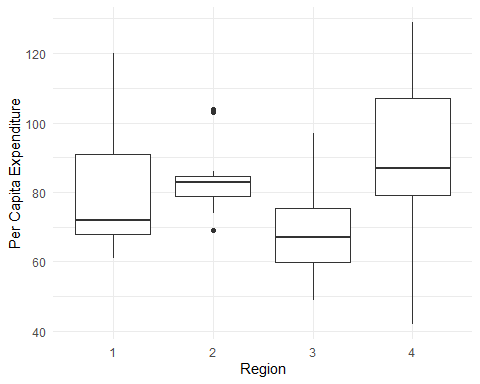
\includegraphics[width=0.8\textwidth]{3}
\end{figure}
\begin{itemize}
	\item \textbf{Result:}
	\item  On average, region 4 has the highest per capita expenditure on housing assistance.
	\\

\end{itemize}
\item
Please plot the relationship between \emph{Y} and \emph{X1}? Describe this graph and the relationship. Reproduce the above graph including one more variable \emph{Region} and display different regions with different types of symbols and colors.
\vspace{.5cm}
\lstinputlisting[language=R, firstline=44, lastline=50]{PS01_Yuanyuan_Liu.R} 
\begin{figure}[H]
	\centering
	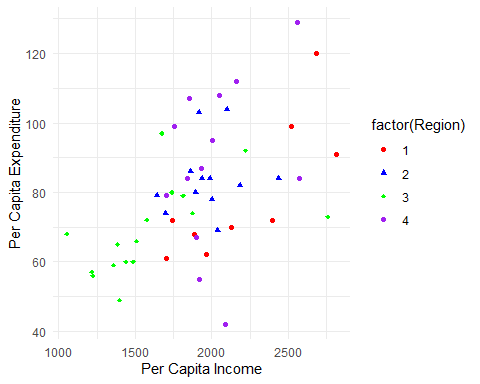
\includegraphics[width=0.8\textwidth]{4}
\end{figure}
\item The x-axis represents the per capita personal income in the state, while the y-axis represents the per capita expenditure on shelters/housing assistance in the state. Different colors and shapes are used to distinguish regions (1 = Northeast, 2 = North Central, 3 = South, 4 = West). 
\begin{itemize}
	\item\textbf{ Result:}
	\item Focusing on Region 3 (South), characterized by its comparatively lower per capita income, it is evident from the chart that a positive correlation exists between per capita personal income (X1) and per capita housing/housing assistance expenditures (Y). Specifically, higher per capita personal income (X1) is associated with higher per capita housing/housing assistance expenditures (Y). Notably, the South region exhibits the lowest per capita personal income (X1) and the lowest per capita housing/housing assistance expenditures (Y).
\end{itemize}
\end{itemize}
\end{document}
